% Chapter 3
%\setstretch{1} 
\chapter{Region based segmentation in presence of inhomogeneity} % Main chapter title
%\setstretch{1.5} 
\label{L2S_Ch} % For referencing the chapter elsewhere, use \ref{Chapter2} 

\lhead{Chapter 5. \emph{L2S}} % This is for the header on each page - perhaps a shortened title

%----------------------------------------------------------------------------------------
In the previous chapter we discussed the potential benefits of using geometric active contours for segmentation problems. Geometric snakes are capable of adapting to the topology of the objects and  their ability to elastically deform and delineate object boundaries with sub-pixel accuracy make these methods attractive choice for several biomedical image analysis applications. 

We have also illustrated how region based models are more suitable for segmenting noisy images with weak edges. One popular region based algorithm is due to Chan and Vese\cite{chan_vese} where the authors model the image as a set of flat zones or regions with constant gray value. The authors also propose a multi-phase variant \cite{vese_multiphase} of their approach to perform multi-class grouping. 

The constant illumination assumption is challenged in applications where the signal intensity is inhomogeneous. This is encountered frequently in many medical and biological imaging applications like magnetic resonance (MR) imaging, ultrasound, X-ray, confocal and electron microscopy, etc. While edge based techniques are better suited for non uniformly illuminated images, low SNR and weak edges of biological structures limit their general applicability.

\section{Application to 2D neuron tracing}

Before dealing with the 3D confocal images, which require more sophisticated processing, we first propose a segmentation algorithm which would work on relatively simpler 2D images. A 2D image is obtained from its 3D counterpart by taking a mean intensity projection along its vertical axis. Although the depth information is lost  when the image dimension is reduced by projecting it to a 2D space, there are several interesting issues which demand our attention even after this simplification. First, even after conversion  2D, we still retain substantial information about a neuron's morphology and this is why there exists a number of popular tracers which have been developed specifically for 2D processing \cite{basu2010tree2tree,meijering2004design}. Also, certain categories of neurons (e.g. the cells in the sub cuticle layer of  the Drosophila) exhibit flat topology, and for such applications 2D processing is more relevant.
Second, with the reduced dimension, one may perform computation at a much faster rate than in 3D, thereby making 2D analysis an attractive choice for an initial, global assessment of the neurites.  Finally, the 2D conversion introduces further challenges for image processing, including introduction of intensity inhomogeneity, which occurs due to signal attenuation by the tissues at greater depths. It is a challenge in itself to investigate the applicability of state of the art segmentation algorithms on these datasets and understand the special processing needs for further robust analysis.

\section{Background and motivation}
In this chapter we introduce an edge oblivious segmentation approach \emph{Legendre Level Set} (L2S), which is robust to smooth variations in region intensity levels. State of the art techniques that tackle inhomogeneity typically require some form of local processing. However, while a global method like Chan-Vese's is insufficient in handling large scale intensity variations, a strictly local approach may lead to undesired segmentation artifacts, especially in presence of noise. We aim to eradicate these issues by proposing a generalized solution for region based segmentation in presence of significant intensity variation and additive noise. 

Chan and Vese's region based technique is mathematically summarized in (\ref{eq:chan_vese}). The locally optimum level set embedding function $\phi^*$ that minimizes (\ref{eq:chan_vese}) partitions the image in two regions such that the foreground and background are best approximated by the scalars $c_1$ and $c_2$, which are computed using alternate minimization.

As mentioned previously, this model is incapable of handling spatially varying illumination. A solution was proposed in \cite{vese_multiphase}, where the authors replaced the scalars $c_1,c_2$  with smooth functions $c_1(\textbf{x})$ and $c_2(\textbf{x})$ in (\ref{eq:chan_vese_PS}).
\bea
\mathcal{E}_{CV}(\phi,c_1(\textbf{x}),c_2(\textbf{x}))&= \displaystyle\int_{\Omega}|f(\textbf{x})-c_1(\textbf{x})|^2\heav(\phi) d\textbf{x} + \int_{\Omega}|f(\textbf{x})-c_2(\textbf{x})|^2\heav(\phi) d\textbf{x} \nn
\\&+\displaystyle s_1\int_{\Omega}|\nabla c_1(\textbf{x})|d\textbf{x} + s_2\int_{\Omega}|\nabla c_2(\textbf{x})|d\textbf{x}
\label{eq:chan_vese_PS}
\eea
Smoothness of the functions are established by regulating their total variation, controlled by the parameters $s_1,s_2$. As before, alternating minimization is used to solve (\ref{eq:chan_vese_PS}). However, unlike (\ref{eq:chan_vese}), the polynomials are computed numerically, by deriving the EL equations and using gradient descent for local minimization.
%\bea
%\dfrac{\partial c_1(\textbf{x})}{\partial t} &=& 2(f(\textbf{x})-c_1(\textbf{x}))\heav
%(\phi) + s_1 \text{div}\left(\dfrac{\nabla c_1(\textbf{x})}{|\nabla c_1(\textbf{x})|}\right) \nn \\
%\dfrac{\partial c_2(\textbf{x})}{\partial t} &=& 2(f(\textbf{x})-c_2(\textbf{x}))\heav(\phi) + s_2 \text{div}\left(\dfrac{\nabla c_2(\textbf{x})}{|\nabla c_2(\textbf{x})|}\right)  \\
%\dfrac{\partial \phi}{\partial t} &=& \left[-(f(\textbf{x})-c_1^*(\textbf{x}))^2+(f(\textbf{x})-c_2^*(\textbf{x}))^2\right]\dirac(\phi) \nn
%\label{eq:PS_solution}
%\eea
\begin{gather}
\dfrac{\partial c_1(\textbf{x})}{\partial t} = 2(f(\textbf{x})-c_1(\textbf{x}))\heav
(\phi) + s_1 \text{div}\left(\dfrac{\nabla c_1(\textbf{x})}{|\nabla c_1(\textbf{x})|}\right) \nn \\
\dfrac{\partial c_2(\textbf{x})}{\partial t} = 2(f(\textbf{x})-c_2(\textbf{x}))\heav(\phi) + s_2 \text{div}\left(\dfrac{\nabla c_2(\textbf{x})}{|\nabla c_2(\textbf{x})|}\right)  \\
\dfrac{\partial \phi}{\partial t} = \left[-(f(\textbf{x})-c_1^*(\textbf{x}))^2+(f(\textbf{x})-c_2^*(\textbf{x}))^2\right]\dirac(\phi) \nn
\label{eq:PS_solution}
\end{gather}
While the solution is attractive, this piecewise smooth model is computationally expensive. This is because, in order to calculate the locally optimum level set function $\phi^*$, one needs to iteratively calculate the functions $c_1^*(\textbf{x})$ and $c_2^*(\textbf{x})$ by numerically solving (\ref{eq:PS_solution}) thereby making computation significantly expensive. 

Recently, Li \textit{et al}. \cite{li_region_scalable} introduced a region scalable model to localize the energy functional. The region localization is controlled by the scale of a Gaussian kernel, which is manually tuned for optimal performance. Efforts have been made to incorporate the region statistics for segmentation \cite{kim_nonparametric,cremers2007review}. These methods are robust to initialization and relatively less sensitive to noise. However, Lankton \textit{et al}.\cite{lankton_localCV} demonstrated that global statistics may not be the best resort for segmenting inhomogeneous objects. Instead, the authors generalize the local region based methods, by proposing a generic energy functional capable of performing segmentation using different region based criteria. 
They also show that by judiciously tuning the region localizing mask size, one can achieve high quality segmentation, even in presence of noise and inhomogeneity. 
However, one downside of their approach is that it requires additional local computation, thus increasing the risk of being stuck within local minima. 


Feng \textit{et al}.  \cite{feng2000tomographic} proposed a method for tomographic reconstruction by using a low order parametric model to represent object texture. However, the algorithm is tailored for tomographic reconstruction and is difficult to generalize. Recently a method was proposed to model the foreground and background by a linear function \cite{du_linear_approx}. This approach is an improvement over the model of Chan-Vese, but does not accommodate nonlinear illumination change.  

From the above discussion we observe that a majority of these approaches rely on local information only. While localizing the segmentation energy is essential in dealing with inhomegeneity, a generic global framework is also necessary to avoid the local minima problem. We propose to model the foreground and background illumination by a set of Legendre basis functions \cite{mukherjee_L2S}. This model allows the region intensities to be represented in a lower dimensional subspace, thereby permitting smooth approximation. Low dimensional signal representation has been used in a slightly different context in the literature, primarily to accommodate shape priors for segmentation \cite{fritscher20073d,huang2008metamorphs}.  However, although shape based information assists segmentation, such techniques require an atlas of pre-registered objects, which may be unavailable for general purpose segmentation. 
We further show that the proposed model \textit{Legendre Level Set} (or L2S) is computationally simple, since we achieve a stable, closed form solution at each iteration, allowing faster processing.

\section{2D segmentation using L2S}

The traditional Chan-Vese functional (\ref{eq:chan_vese}) can be reformulated and generalized by replacing the scalars $c_1$ and $c_2$ by   smooth functions $c_1^m(\textbf{x})$ and $c_2^m(\textbf{x})$. These functions are used to model the intensity in the two regions separated by the zero level set curves of $\phi$. The energy functional corresponding to the L2S data term is expressed as follows:
\bea
\mathcal{E}_{L2S}= \int_{\Omega}|f(\textbf{x})-c_1^m(\textbf{x})|^2H(\phi) d\textbf{x} 
						   +\int_{\Omega}|f(\textbf{x})-c_2^m(\textbf{x})|^2 \left(1-H(\phi)\right) d\textbf{x}  
\label{eq:L2S_data}
\eea
The essence of our approach is embedded in computing these functions. By allowing the regions to be modeled by flexible (but smooth) functions, we introduce the local information required to tackle the heterogeneous illumination. This is a notable feature of our algorithm. Unlike (\ref{eq:chan_vese_PS}), where smoothness is obtained by minimizing the total variation term, we only allow inherently smooth polynomials to approximate the region intensities. As we will show in the next few sections, this formulation allows a suitable framework to model the heterogeneity, without significantly sacrificing on computational time.

To preserve the smoothness and flexibility of the functions, we represent them as a linear combination of a few Legendre basis functions as shown below:
\bea
 c_1^m(\textbf{x}) &=& \sum_{k=0}^m\alpha_k\mathcal{P}_k(\textbf{x}) \\ c_2^m(\textbf{x}) &=& \sum_{k=0}^m\beta_k\mathcal{P}_k(\textbf{x})
 \label{eq:l2s_poly}
\eea
Here $\mathcal{P}_k$ is a multidimensional Legendre polynomial, which can be written as the outer product of the one dimensional counterparts. The 2-D polynomial is computed as $\mathcal{P}_k(x,y)=p_k(x)p_k(y)$, $\textbf{x}=(x,y)\in \Omega \subset [-1,1]^2$. $p_k$ is a one dimensional Legendre polynomial of degree $k$ defined as
\bea
p_k(x)=	\frac{1}{2^k}\sum_{i=0}^{k}\binom{k}{i}(x-1)^{k-i}(x+1)^i  
\label{eq:legendre}
\eea
The highest degree of the 1D bases is denoted by $m$. Hence, for the 2D case, we would represent the regions by a linear combination of a set of $(m+1)^2$ 2D Legendre basis functions.

\subsection{Optimization of the energy functional}
\begin{figure}[ht]
\centering
\captionsetup{justification=centering}
\renewcommand{\tabcolsep}{0.05cm}
\begin{tabular}{@{}ccc @{}}
	
\includegraphics[width=.3\textwidth]{./images/Bases_color/1}  &
	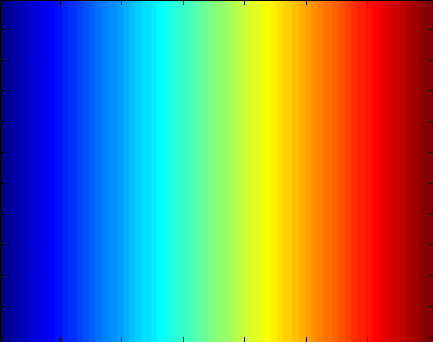
\includegraphics[width=.3\textwidth]{./images/Bases_color/2}  &
	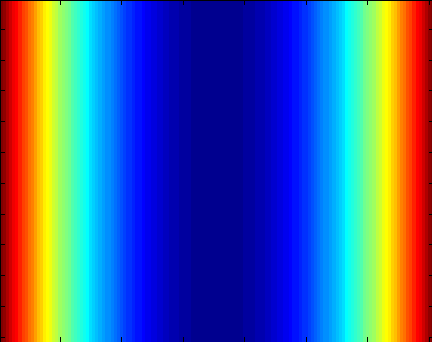
\includegraphics[width=.3\textwidth]{./images/Bases_color/3}  \\
	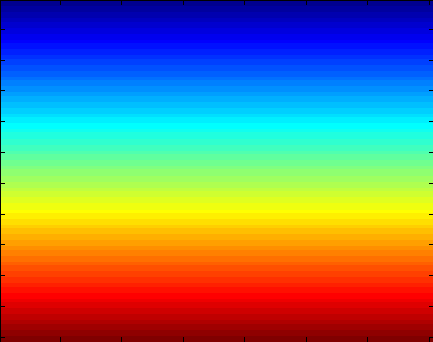
\includegraphics[width=.3\textwidth]{./images/Bases_color/4}  &
	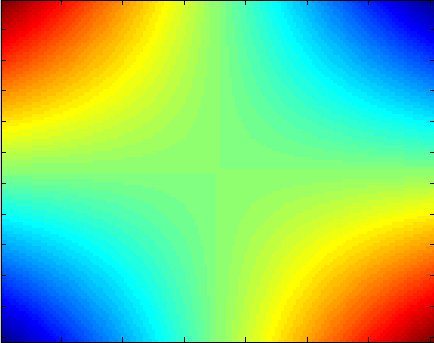
\includegraphics[width=.3\textwidth]{./images/Bases_color/5}  &
	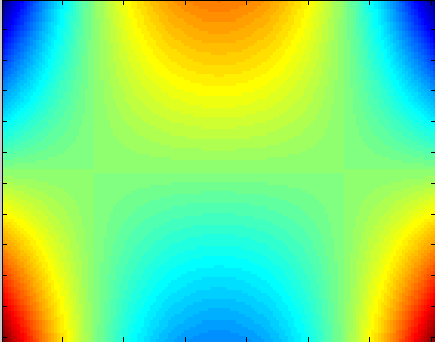
\includegraphics[width=.3\textwidth]{./images/Bases_color/6}  \\
	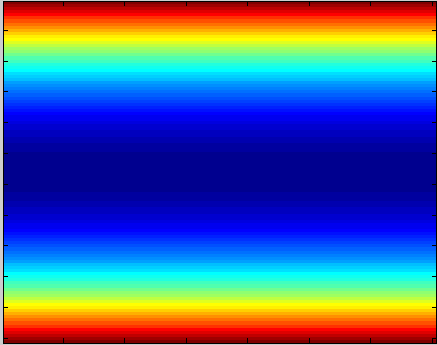
\includegraphics[width=.3\textwidth]{./images/Bases_color/7}  &
	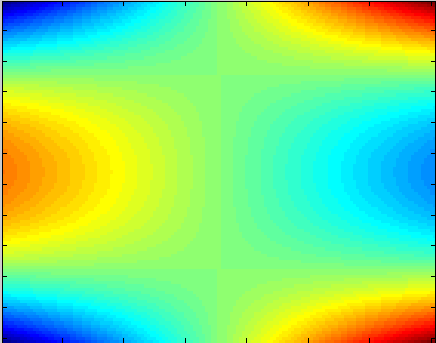
\includegraphics[width=.3\textwidth]{./images/Bases_color/8}  &
	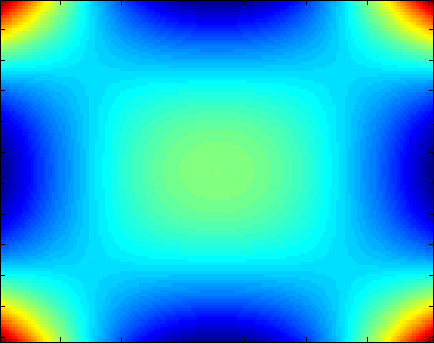
\includegraphics[width=.3\textwidth]{./images/Bases_color/9} 
\end{tabular}
\caption[2D Legendre polynomials]{The set of nine 2D Legendre basis functions. The 2D polynomials are computed from 1D functions of degree 2.}
\label{fig:legendre_bases}
\end{figure}

Let us denote $\mathbb{P}(\textbf{x})=\left(\mathcal{P}_0(\textbf{x}),\ldots, \mathcal{P}_{N-1}(\textbf{x})\right)^T$ as the vector of Legendre polynomials. $\textbf{a}=\left(\alpha_0,\ldots,\alpha_{N-1} \right)^T$ and $\textbf{b}=\left(\beta_0,\ldots,\beta_{N-1} \right)^T$ are the coefficient vectors for the two regions. $N=(m+1)^2$ is the total number of basis functions. We can now rewrite the modified version of (\ref{eq:chan_vese}) in matrix form as
\bea
\mathcal{E}(\phi,\textbf{a},\textbf{b})&= \displaystyle\int_{\Omega}\left[|f(\textbf{x})-\textbf{a}^T\mathbb{P}(\textbf{x})|^2 m_1(\textbf{x})+|f(\textbf{x})-\textbf{b}^T\mathbb{P}(\textbf{x})|^2m_2(\textbf{x}) \right]d\textbf{x} \nn \\
						    &+\lambda_1 ||\textbf{a}||_2^2  +\lambda_2 ||\textbf{b}||_2^2 + \nu\, \lint_{\Omega} |\nabla\heav(\phi)| d\textbf{x} 
\label{eq:leg_cv_mat}						  
\eea
In (\ref{eq:leg_cv_mat}) the last term introduces smoothness in the zero level curve, which is regulated by the parameter $\nu$.  Let us also denote  $m_1(\textbf{x})=\heav(\phi)$ and  $m_2(\textbf{x})=1-m_1(\textbf{x})$. 


The non negative regularizing parameters $\lambda_1,\lambda_2$ can be selected using cross validation techniques to avoid over-fitting.
The energy functional (\ref{eq:leg_cv_mat}) is optimized using alternating minimization. In the first step, to find the optimal coefficients, we take the partial derivative of (\ref{eq:leg_cv_mat}) with respect to $\textbf{a}$ and $\textbf{b}$ respectively and setting the result to zero. A closed form solution $\hat{\textbf{a}}$ and $\hat{\textbf{b}}$ is obtained as
\bea
\dfrac{\partial\mathcal{E}(\phi,\textbf{a},\textbf{b})}{\partial \textbf{a}}=0 \Rightarrow \hat{\textbf{a}} =& \left[K+ \lambda_1 \mathbb{I}\right]^{-1}\textbf{p} \\
\dfrac{\partial\mathcal{E}(\phi,\textbf{a},\textbf{b})}{\partial \textbf{b}}=0 \Rightarrow \hat{\textbf{b}} =& \left[L+ \lambda_2 \mathbb{I}\right]^{-1}\textbf{q} 
\label{coef_sol}
\eea
$\left[. \right]$ denotes a matrix. 
Here $\left[K \right]$ and $\left[L \right]$ are Gramian matrices \cite{gramian} of dimension $N\times N$, whose $(i,j)^{th}$ entry are obtained as follows:
\bea
\left[K\right]_{i,j}=& \left<\sqrt{m_1(\textbf{x})}\mathcal{P}_i(\textbf{x}),\sqrt{m_1(\textbf{x})}\mathcal{P}_j(\textbf{x})\right>=&\displaystyle \int_{\Omega}m_1(\textbf{x})\mathcal{P}_i(\textbf{x})\mathcal{P}_j(\textbf{x})d\textbf{x} \\
\left[L\right]_{i,j}=& \left<\sqrt{m_2(\textbf{x})}\mathcal{P}_i(\textbf{x}),\sqrt{m_2(\textbf{x})}\mathcal{P}_j(\textbf{x})\right>=&\displaystyle \int_{\Omega}m_2(\textbf{x})\mathcal{P}_i(\textbf{x})\mathcal{P}_j(\textbf{x})d\textbf{x}
\eea
Here $\left<,\right>$ denotes the inner product operator for real valued functions, and $0\leq i,j \leq N$. The individual elements $p_j$ and $q_j$ of the $N\times 1$ vectors  $\textbf{p}=\left(p_0,\ldots,p_N\right)^T$ and $\textbf{q}=\left(q_0,\ldots,q_N\right)^T$ are obtained as 
$
p_j=\lint_{\Omega} \mathcal{P}_j(\textbf{x})f(\textbf{x})m_1(\textbf{x})d\textbf{x} 
$ and 
$q_j =\lint_{\Omega} \mathcal{P}_j(\textbf{x})f(\textbf{x})m_2(\textbf{x})d\textbf{x}$ .
This can be written in a more compact form using vector notations as follows:
\bea
\textbf{p}=\lint_{\Omega} \mathbb{P}(\textbf{x})f(\textbf{x})m_1(\textbf{x})d\textbf{x} \label{eq:l2s_P}
\\
\textbf{q} =\lint_{\Omega} \mathbb{P}(\textbf{x})f(\textbf{x})m_2(\textbf{x})d\textbf{x}
\label{eq:l2s_Q}
\eea
With the updated coefficient vectors, we can now locally minimize (\ref{eq:leg_cv_mat}) with respect to $\phi$ borrowing techniques from variational calculus. 
The curve evolution is performed by numerically solving the following partial differential equation:
\bea
\frac{\partial \phi}{\partial t}=& \left[-|f(\textbf{x})-\hat{\textbf{a}}^T\mathbb{P}(\textbf{x})|^2 
						   +|f(\textbf{x})-\hat{\textbf{b}}^T\mathbb{P}(\textbf{x})|^2  + \nu \, \nabla \cdot\left(\dfrac{\nabla\phi}{|\nabla\phi|}\right) \right]\dirac(\phi)\nn\\
\label{eq:l2s_gradient_flow}
\eea
We solve (\ref{eq:l2s_gradient_flow}) using gradient descent and initializing $\phi|_{t=0}=\phi_0$ and $\dfrac{\dirac(\phi)}{|\nabla \phi|}\dfrac{\partial\phi}{\partial \hat{n}}=0$ at the domain boundary. See Appendix \ref{AppendixTuFF} for derivation of (\ref{eq:l2s_gradient_flow}).

\subsection{Analysis of L2S}
The surface approximate for foreground and background are obtained by computing $\hat{\textbf{a}}^T\mathbb{P}(\textbf{x})$ and $\hat{\textbf{b}}^T\mathbb{P}(\textbf{x})$. Since the coefficient vectors are available in closed form, it makes our algorithm fast and effective. The amount of intensity variation is governed by the coefficient vectors which are computed automatically. However, computing the coefficient vectors require a matrix inversion step. Here we show that the matrices $\left[K\right]$ and $\left[L\right]$ are invertible when the heaviside function is suitably regularized.

Since $\left[K\right]$ is a Gramian matrix, it is full rank iff the polynomials $\sqrt{m_1(\textbf{x})}\mathcal{P}_i(\textbf{x})$, $(i=1,\ldots,N)$ are linearly independent \cite{gramian}. Since the polynomials $\mathcal{P}_i(\textbf{x})$ are linearly independent themselves, it is easy to show that the linear independence holds if $0< m_1(\textbf{x})< 1$. A similar argument holds for analyzing the invertibility of $\left[L\right]$. In \cite{chan_vese}, the authors propose a regularized version of the heaviside function which is given by (\ref{eq:heav_relax})
By this definition, the functions $m_1(\textbf{x})$ and $m_2(\textbf{x})$ are bounded in $\left[0,1\right]$, which make the matrices invertible. 

However, inverting the above mentioned matrices may still be prone to numerical error  when $\sqrt{m_i(\textbf{x})}$ is small. The regularizing constants $\lambda_1$ and $\lambda_2$ contribute to make these matrices well conditioned. Furthermore, the regularization terms are necessary to avoid over-fitting. In most situations, we find that only a few (typically 16) 2-D Legendre functions are sufficient to model the region intensity. However, image noise may lead to over-fitting of the polynomials to the image segments, which may disrupt segmentation as the propagating level set may settle at a local minima. The scalars $\lambda_1,\lambda_2$ produce a damping effect by constraining the $\mathbb{L}_2$ norm of the bases coefficients, thereby favoring interior regions approximated by smooth functions. 

\subsection{Parameter selection for L2S}
Our algorithm requires specification of a few parameters, namely the Legendre polynomial degree $m$ and the regularizing constants $\lambda_1$ and $\lambda_2$ in (\ref{eq:leg_cv_mat}). We experimentally verified that the intensity variation in the images can be adequately modeled by using 1-D Legendre polynomials of (highest) degree three. We found that the algorithm is relatively robust to the selection of this value, but a higher degree polynomial typically requires inversion of a larger matrix, which makes computation significantly more expensive. To estimate the value of $\lambda_1$ and $\lambda_2$, we perform a \textit{leave one out} cross validation on each of the four categories in our dataset. The cross validation is performed over the values of $\{0,1,\ldots,100\}$ in multiples of 2. For simplicity, we have chosen $\lambda_1=\lambda_2$ for every experiment. The particular value which yields the highest average Dice coefficient for each dataset is chosen for experimentation. 


Automated selection of the contour smoothness parameter $\nu$ in (\ref{eq:leg_cv_mat}) is non-trivial. Typically, $0<\nu<1$, where a higher value produces smoother contour. As a rule of thumb, one may wish to set $\nu$ to a relatively higher value if the noise level in the image is high. For our experiments, we observe that the set of ultrasound images and the simulated noisy images require larger values of $\nu$. For all these images, we select $\nu=0.6$. For the less noisy images, $\nu$ is typically set in the range 0.05 to 0.2. 
 
\subsection{Comparison with GAC and Chan-Vese}
In Chapter 4, we introduced the edge based geodesic active contour\cite{caselles_geodesic} model and region based technique due to Chan and Vese \cite{chan_vese}. Fig.~\ref{fig:l2s_compare_GAC_CV} shows the performance of L2S versus GAC and Chan-Vese's method. To maintain fairness of comparison, we have initialized the level set at the same positions for each methods (shown by the green contour). All the five images used for this demonstration are characterized by low contrast, weak edges and significant variation in region illumination levels. 
\begin{figure}[t]
\centering
\renewcommand{\tabcolsep}{0.05cm}
\begin{tabular}{@{}cccc@{}}

\includegraphics[width=0.24\textwidth]{images/L2S_compare/orig_2}	&
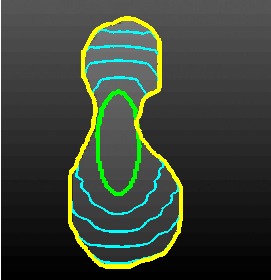
\includegraphics[width=0.24\textwidth]{images/L2S_compare/GAC_2}	&
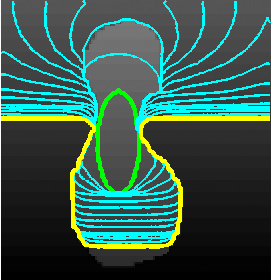
\includegraphics[width=0.24\textwidth]{images/L2S_compare/CV_2}		&
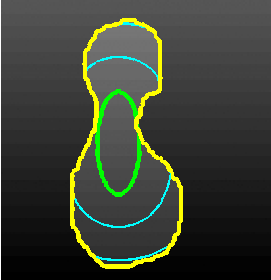
\includegraphics[width=0.24\textwidth]{images/L2S_compare/L2S_2}	
%\\
%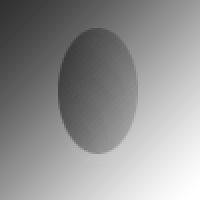
\includegraphics[width=0.24\textwidth]{images/L2S_compare/orig_3}	&
%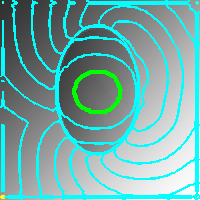
\includegraphics[width=0.24\textwidth]{images/L2S_compare/GAC_3}	&
%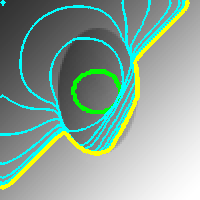
\includegraphics[width=0.24\textwidth]{images/L2S_compare/CV_3}		&
%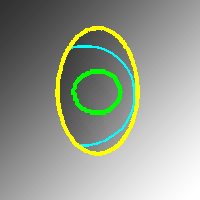
\includegraphics[width=0.24\textwidth]{images/L2S_compare/L2S_3}	
\\
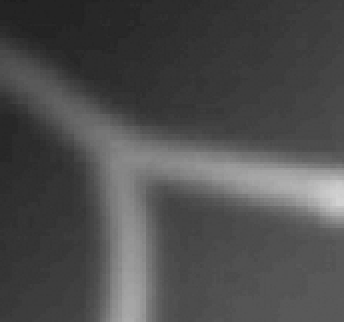
\includegraphics[width=0.24\textwidth]{images/L2S_compare/orig_1}	&
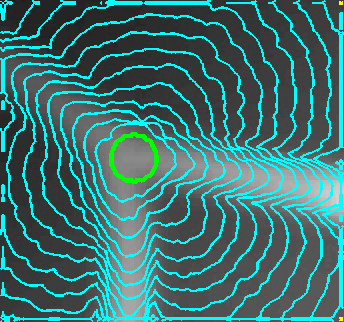
\includegraphics[width=0.24\textwidth]{images/L2S_compare/GAC_1}	&
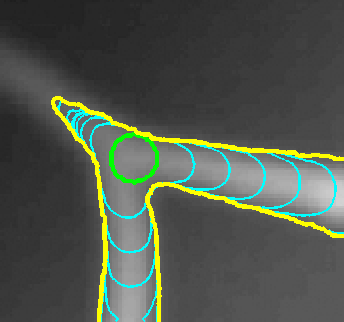
\includegraphics[width=0.24\textwidth]{images/L2S_compare/CV_1}		&
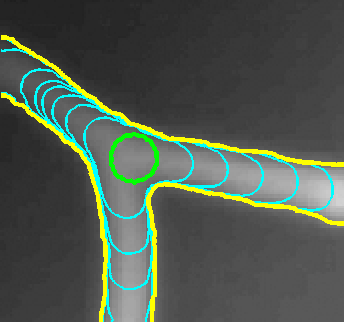
\includegraphics[width=0.24\textwidth]{images/L2S_compare/L2S_1}	
\\
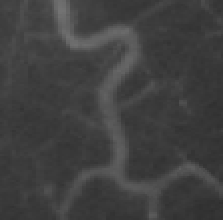
\includegraphics[width=0.24\textwidth]{images/L2S_compare/orig_4}	&
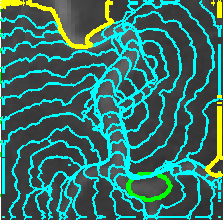
\includegraphics[width=0.24\textwidth]{images/L2S_compare/GAC_4}	&
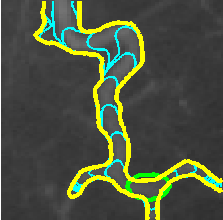
\includegraphics[width=0.24\textwidth]{images/L2S_compare/CV_4}		&
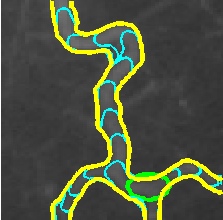
\includegraphics[width=0.24\textwidth]{images/L2S_compare/L2S_4}	
\\
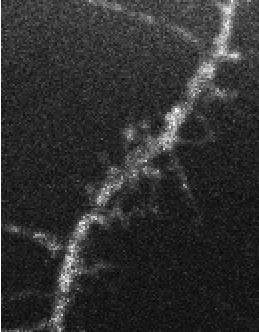
\includegraphics[width=0.24\textwidth]{images/L2S_compare/orig_5}	&
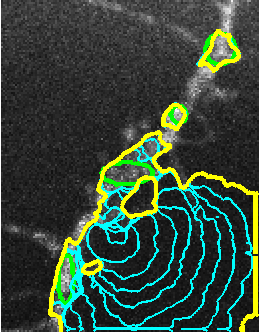
\includegraphics[width=0.24\textwidth]{images/L2S_compare/GAC_5}	&
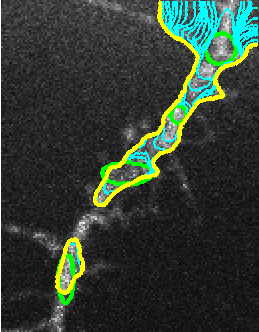
\includegraphics[width=0.24\textwidth]{images/L2S_compare/CV_5}		&
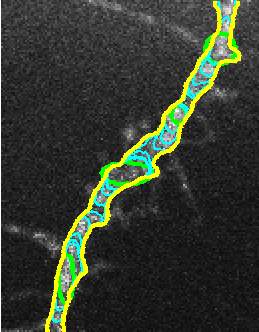
\includegraphics[width=0.24\textwidth]{images/L2S_compare/L2S_5}	\\
(a) original image & (b) GAC & (c) Chan Vese & (d) L2S
\end{tabular}
\caption[L2S vs GAC vs Chan-Vese]{(a) A 2D image. Segmentation via (b) Geodesic active contour, (c)Chan-Vese and (d)L2S. The initial contour is plotted in green and the final contour in yellow. Intermediate steps of curve evolution are shown in cyan. Best viewed in color.}
\label{fig:l2s_compare_GAC_CV}
\end{figure}
GAC and Chan-Vese's algorithm's performance is limited due to these artifacts. GAC is prone to error due to weak edges causing contour leakage, whereas the piecewise constant model due to Chan and Vese is unable to accomodate the intensity inhomogeneities. However, we observe that L2S exhibits significantly superior qualitative performance since it is (a) not dependent on the edge information and (b) capable of handling discontinuities by using polynomial approximation for region intensities.

%\clearpage
\subsection{Comparison with other methods}
To demonstrate the efficacy of the proposed method, we perform further experiments on a dataset of 32 images. The dataset consists of a set of synthetic images with added noise and simulated intensity inhomogeneity, a set of biomedical images consisting of blood vessels using magnetic resonance angiogram (MRA), neurons and dendritic spines imaged by confocal microscope and finally, a set of ultrasound images of human blood vessels.  

To evaluate the performance of L2S, we compare our approach with three popular and widely used region based segmentation algorithms viz. Chan-Vese \cite{chan_vese}, Lankton et. al. \cite{lankton_localCV} and Li et. al.\cite{li_region_scalable}. We use the freely available CREASEG\cite{creaseg} tool to evaluate the performance. We choose the above techniques for performance evaluation since all the above models (barring Chan-Vese) were developed to perform region based segmentation with varying object brightness.

To set up the comparative evaluation procedure, we first present the segmentation results on a biomedical image dataset containing vascular structures. This is shown in Fig.~\ref{fig:l2s_compare_vessels}. Fig.~\ref{fig:l2s_compare_vessels}(a) shows the original microscopy images with the initial contour shown in yellow, followed by segmentation results due to (b) Chan-Vese in blue, (c) Lankton \textit{et al.} in red, (d) Li \textit{et al.} in cyan and finally (e) L2S (yellow). The images contains vascular structures and are characterized by  noise, non-object clutter and inhomogeneous intensity. To make a fair evaluation, the images were not preprocessed for contrast improvement or noise removal. 
\begin{figure*}[t]
\centering
\renewcommand{\tabcolsep}{0.05cm}
\begin{tabular}{@{}ccccc@{}}
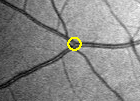
\includegraphics[width=0.19\textwidth]{images/L2S_compare_region/19_orig}	&
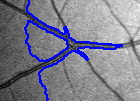
\includegraphics[width=0.19\textwidth]{images/L2S_compare_region/19_CV}	&
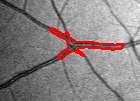
\includegraphics[width=0.19\textwidth]{images/L2S_compare_region/19_Lankton}		&
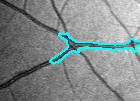
\includegraphics[width=0.19\textwidth]{images/L2S_compare_region/19_Li}	&
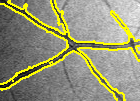
\includegraphics[width=0.19\textwidth]{images/L2S_compare_region/19_ours}	
\\
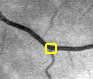
\includegraphics[width=0.19\textwidth]{images/L2S_compare_region/22_trng_orig}	&
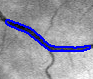
\includegraphics[width=0.19\textwidth]{images/L2S_compare_region/22_trng_CV}	&
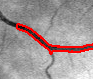
\includegraphics[width=0.19\textwidth]{images/L2S_compare_region/22_trng_Lankton}		&
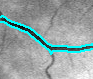
\includegraphics[width=0.19\textwidth]{images/L2S_compare_region/22_trng_Li}	&
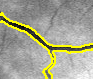
\includegraphics[width=0.19\textwidth]{images/L2S_compare_region/22_trng_ours}	
\\
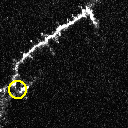
\includegraphics[width=0.19\textwidth]{images/L2S_compare_region/dendrites2_orig}	&
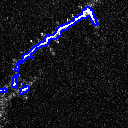
\includegraphics[width=0.19\textwidth]{images/L2S_compare_region/dendrites2_CV}	&
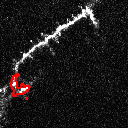
\includegraphics[width=0.19\textwidth]{images/L2S_compare_region/dendrites2_Lankton} &
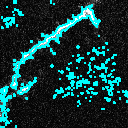
\includegraphics[width=0.19\textwidth]{images/L2S_compare_region/dendrites2_Li}	&
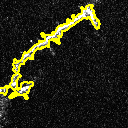
\includegraphics[width=0.19\textwidth]{images/L2S_compare_region/dendrites2_ours}	
\\
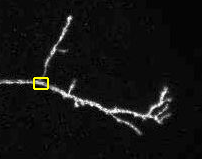
\includegraphics[width=0.19\textwidth]{images/L2S_compare_region/n13_orig}	&
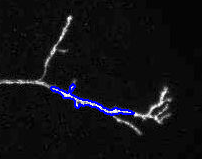
\includegraphics[width=0.19\textwidth]{images/L2S_compare_region/n13_CV}	&
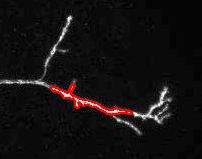
\includegraphics[width=0.19\textwidth]{images/L2S_compare_region/n13_Lankton} &
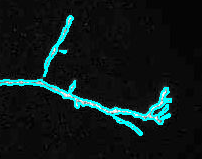
\includegraphics[width=0.19\textwidth]{images/L2S_compare_region/n13_Li}	&
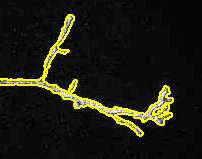
\includegraphics[width=0.19\textwidth]{images/L2S_compare_region/n13_ours}	
\\
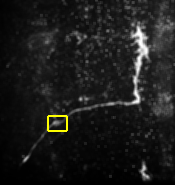
\includegraphics[width=0.19\textwidth]{images/L2S_compare_region/neuron_clear_orig}	&
\includegraphics[width=0.19\textwidth]{images/L2S_compare_region/neuron_clear_CV}	&
\includegraphics[width=0.19\textwidth]{images/L2S_compare_region/neuron_clear_Lankton} &
\includegraphics[width=0.19\textwidth]{images/L2S_compare_region/neuron_clear_Li}	&
\includegraphics[width=0.19\textwidth]{images/L2S_compare_region/neuron_clear_ours}	
\\
\includegraphics[width=0.19\textwidth]{images/L2S_compare_region/spine2_orig}	&
\includegraphics[width=0.19\textwidth]{images/L2S_compare_region/spine2_CV}	&
\includegraphics[width=0.19\textwidth]{images/L2S_compare_region/spine2_Lankton} &
\includegraphics[width=0.19\textwidth]{images/L2S_compare_region/spine2_Li}	&
\includegraphics[width=0.19\textwidth]{images/L2S_compare_region/spine2_ours}	
\\
\includegraphics[width=0.19\textwidth]{images/L2S_compare_region/Vessel_CTA1_orig}&
\includegraphics[width=0.19\textwidth]{images/L2S_compare_region/Vessel_CTA1_CV}	&
\includegraphics[width=0.19\textwidth]{images/L2S_compare_region/Vessel_CTA1_Langton} &
\includegraphics[width=0.19\textwidth]{images/L2S_compare_region/Vessel_CTA1_Li}	&
\includegraphics[width=0.19\textwidth]{images/L2S_compare_region/Vessel_CTA1_ours}	
\\
\includegraphics[width=0.19\textwidth]{images/L2S_compare_region/vessel1_orig}	&
\includegraphics[width=0.19\textwidth]{images/L2S_compare_region/vessel1_CV}	&
\includegraphics[width=0.19\textwidth]{images/L2S_compare_region/vessel1_Lankton} &
\includegraphics[width=0.19\textwidth]{images/L2S_compare_region/vessel1_Li}	&
\includegraphics[width=0.19\textwidth]{images/L2S_compare_region/vessel1_ours}	
\\
\scriptsize(a)2D image&\scriptsize(b)Chan-Vese&\scriptsize(c)Lankton \textit{et al}\cite{lankton_localCV}&\scriptsize(d)Li \textit{et al}\cite{li_region_scalable}&\scriptsize(e)L2S
\end{tabular}
\caption[L2S on vascular images]{Qualitative comparison of L2S for vascular images.}
\label{fig:l2s_compare_vessels}
\end{figure*}
\clearpage

\begin{figure*}[t]
\centering
\renewcommand{\tabcolsep}{0.05cm}
\begin{tabular}{@{}ccccc@{}}
\includegraphics[width=0.19\textwidth]{images/L2S_compare_region/Degrade_orig}	&
\includegraphics[width=0.19\textwidth]{images/L2S_compare_region/Degrade_CV}	&
\includegraphics[width=0.19\textwidth]{images/L2S_compare_region/Degrade_Lankton}		&
\includegraphics[width=0.19\textwidth]{images/L2S_compare_region/Degrade_Li}	&
\includegraphics[width=0.19\textwidth]{images/L2S_compare_region/Degrade_ours}	
\\
\includegraphics[width=0.19\textwidth]{images/L2S_compare_region/SIM2_orig}	&
\includegraphics[width=0.19\textwidth]{images/L2S_compare_region/SIM2_CV}	&
\includegraphics[width=0.19\textwidth]{images/L2S_compare_region/SIM2_Lankton}		&
\includegraphics[width=0.19\textwidth]{images/L2S_compare_region/SIM2_Li}	&
\includegraphics[width=0.19\textwidth]{images/L2S_compare_region/SIM2_ours}	
\\
\includegraphics[width=0.19\textwidth]{images/L2S_compare_region/mushroom_orig}	&
\includegraphics[width=0.19\textwidth]{images/L2S_compare_region/mushroom_CV}	&
\includegraphics[width=0.19\textwidth]{images/L2S_compare_region/mushroom_Lankton} &
\includegraphics[width=0.19\textwidth]{images/L2S_compare_region/mushroom_Li}	&
\includegraphics[width=0.19\textwidth]{images/L2S_compare_region/mushroom_ours}	
\\
\includegraphics[width=0.19\textwidth]{images/L2S_compare_region/Airplane_orig}	&
\includegraphics[width=0.19\textwidth]{images/L2S_compare_region/Airplane_CV}	&
\includegraphics[width=0.19\textwidth]{images/L2S_compare_region/Airplane_Lankton} &
\includegraphics[width=0.19\textwidth]{images/L2S_compare_region/Airplane_Li}	&
\includegraphics[width=0.19\textwidth]{images/L2S_compare_region/Airplane_ours}	
\\
\includegraphics[width=0.19\textwidth]{images/L2S_compare_region/muscle_orig}	&
\includegraphics[width=0.19\textwidth]{images/L2S_compare_region/muscle_CV}	&
\includegraphics[width=0.19\textwidth]{images/L2S_compare_region/muscle_Lankton}		&
\includegraphics[width=0.19\textwidth]{images/L2S_compare_region/muscle_Li}	&
\includegraphics[width=0.19\textwidth]{images/L2S_compare_region/muscle_ours}	
\\
\includegraphics[width=0.19\textwidth]{images/L2S_compare_region/US3_orig}	&
\includegraphics[width=0.19\textwidth]{images/L2S_compare_region/US3_CV}	&
\includegraphics[width=0.19\textwidth]{images/L2S_compare_region/US3_Lankton} &
\includegraphics[width=0.19\textwidth]{images/L2S_compare_region/US3_Li}	&
\includegraphics[width=0.19\textwidth]{images/L2S_compare_region/US3_ours}	
\\
\includegraphics[width=0.19\textwidth]{images/L2S_compare_region/US7_orig}	&
\includegraphics[width=0.19\textwidth]{images/L2S_compare_region/US7_CV}	&
\includegraphics[width=0.19\textwidth]{images/L2S_compare_region/US7_Lankton} &
\includegraphics[width=0.19\textwidth]{images/L2S_compare_region/US7_Li}	&
\includegraphics[width=0.19\textwidth]{images/L2S_compare_region/US7_ours}	
\\
\includegraphics[width=0.19\textwidth]{images/L2S_compare_region/yeast_orig}	&
\includegraphics[width=0.19\textwidth]{images/L2S_compare_region/yeast_CV}	&
\includegraphics[width=0.19\textwidth]{images/L2S_compare_region/yeast_Lankton} &
\includegraphics[width=0.19\textwidth]{images/L2S_compare_region/yeast_Li}	&
\includegraphics[width=0.19\textwidth]{images/L2S_compare_region/yeast_ours}\\
\scriptsize(a)2D image&\scriptsize(b)Chan-Vese&\scriptsize(c)Lankton \textit{et al}\cite{lankton_localCV}&\scriptsize(d)Li \textit{et al}\cite{li_region_scalable}&\scriptsize(e)L2S
\end{tabular}
\caption[L2S on vascular images]{Qualitative comparison of L2S for non vascular images.}
\label{fig:l2s_compare_nonvessel}
\end{figure*}
\clearpage
We had mentioned earlier that one of our goals is to develop a segmentation procedure which is reasonably widely applicable. In this chapter we do not assume any structural prior for the objects to be segmented. Although prior information may achieve better results, the algorithm loses its general applicability. In the following chapter we will present a more problem specific solution to neuron segmentation. Since L2S is a general purpose segmentation algorithm, we also present qualitative results on non-vascular structures. However, almost all these images are characterized by inhomogeneous contrast, which is the major issue we try to address in this chapter. 

Segmentation results on a few representative images are  shown in Fig.~\ref{fig:l2s_compare_nonvessel}. This set of non vessel images belong to different categories. The first two images are simulated to contain a varying contrast and additive noise. We also include MRI images of human leg muscles, natural images from the Berkeley segmentation database\cite{BerkeleySegDatabase}, noisy ultrasound images of human arteries and finally microscopy images of yeast cells. As before, L2S results are shown in yellow and qualitative comparison suggest robustness of the method.

\subsection{Quantitative performance evaluation}
The Dice coefficient \cite{bernard_splinedCV} is used to quantify the results of segmentation. The Dice index $\mathcal{D}\in [0,1]$ between two regions $R_1$ and $R_2$ is given by 
\bea
\mathcal{D}(R_1,R_2)=2\dfrac{|R_1\cap R_2|}{|R_1|+|R_2|}
\label{eq:Dice}
\eea
Here $R_2$ is a binary image that denotes ground truth segmentation, and $R_1$ is the result obtained experimentally. A Dice index of 1 indicates perfect segmentation. The quantitative performance is shown in Fig.~\ref{fig:L2S_Dice}. 
\begin{figure}[t]
\centering
\includegraphics[width=1\textwidth]{images/L2S_Dice}
\caption[Quantitative comparison of L2S]{Dice index for the different algorithms are plotted in this bar chart. L2S results are shown by the yellow bar. Best viewed in color.}	
\label{fig:L2S_Dice}
\end{figure}
We observe that over this entire dataset, L2S yields an average Dice score of $0.9$, compared to $0.62,0.57$ and $0.7$ for the methods described in \cite{chan_vese},\cite{lankton_localCV} and \cite{li_region_scalable} respectively. 

\subsection{Computational comparison}
\begin{figure}[b]
\centering
\includegraphics[width=0.8\textwidth]{images/L2S_time}
\caption[Computational comparison for L2S]{The CPU running times (sec) for the different algorithms are plotted in this bar chart. L2S results are shown by the yellow bar. Best viewed in color.}	
\label{fig:L2S_comput}
\end{figure}
Our algorithm is implemented in Matlab and all experiments are performed on an Intel Pentium processor with 16 GB memory. The convergence times (in seconds) for the four algorithms are presented in Fig.~\ref{fig:L2S_comput}. Computationally, our method outperforms  \cite{lankton_localCV} and \cite{li_region_scalable} on average. It may be noted that the apparent low convergence time of \cite{chan_vese} often is a result of  convergence at local minima, which do not necessarily correspond to correct object boundaries.

\section{Discussion}
A novel framework for segmentation in presence of significant intra-region illumination variation is presented. Qualitative and quantitative results and comparison with the state of the art techniques suggest robustness of our approach. Here we have focused on bi-level segmentation, although extension to a multi-level framework appears straightforward. Also, our formulation allows easy incorporation of \textit{a priory} shape information, which may enhance performance in select cases. Salient highlights of L2S are presented below:
\begin{itemize}
\item L2S uses geometric active contours for segmentation. Therefore, it can adapt to the topological variations in objects via automatic merging and splitting.
\item L2S is robust against inhomogeneous intensity levels caused by non uniform signal attenuation or external bias fields, which occurs in many biological imaging applications. 
\item L2S is a region based method and its performance is robust against noise and weak edges.
\item L2S is computationally efficient and numerically stable.
\end{itemize}
However, like most level set methods, L2S is somewhat biased towards contour initialization. 
Also, although Legendre polynomials for region intensity approximation provides an elegant solution, it is difficult to comment on the optimality of this choice of bases. Effectiveness of other polynomials such as splines or wavelets \cite{achuthan2010wavelet} needs further investigation. In select cases, it may also be possible to learn a compact set of bases for representation. To address this issue, we identified a scenario  where a set of training examples of the object is available. We show that in such applications, the region approximating polynomials may be learned efficiently, instead of pre specifying them. This segmentation algorithm, \textit{Dictionary Learning Level Sets} (DL2S)\cite{sarkar_DL2S}, leverages the power of dictionary learning\cite{elad_ksvd} to learn the region approximating polynomials. We provide the details of DL2S in Appendix~\ref{AppendixDL2S}.

To develop a customized solution specifically for neuron tracing, we hypothesize that robust performance can be achieved by incorporating prior knowledge about the local shape of the neurites. While L2S is a general purpose, region based technique, in the following chapter we design a solution using level sets, that uses the local tubularity of the neurites to perform curve evolution.
